\documentclass[12 pt, a4paper]{article}
\usepackage[english]{babel}  								% For norsk oppsett
\usepackage[utf8]{inputenc}
\usepackage{amsmath}
\usepackage{amssymb}
\usepackage{graphicx}
\usepackage{tabularx}
\usepackage{subcaption}
\usepackage{hyperref}
\usepackage{fancyhdr}
\usepackage{enumerate}
\usepackage{float}
\usepackage{tikz}
\usepackage{fancyhdr}
\usepackage{lastpage}
\usepackage{circuitikz}
\usepackage{physics}
\usepackage[includeheadfoot, margin =0.5 in]{geometry}
\usepackage[FYS, OnlyFrontpage]{mnfrontpage} 			%SKIFT HER!!!
\usepackage[version=3]{mhchem}
\usepackage{biblatex}%,style=numeric-comp
%\usepackage{cite}
\usepackage{siunitx}
\usepackage{todonotes}
\usepackage{xcolor}
\usepackage{listings}
%%%%
\usepackage[bottom]{footmisc}
\renewcommand\footnoterule{\rule{\linewidth}{0.5pt}}
%\renewcommand[\footnoterule]{%
%	\kern -3pt
%	\hrule width \textwidth height 1pt
%	\kern 2pt
%}
%%%%
\lstset{basicstyle=\ttfamily,
  showstringspaces=false,
  commentstyle=\color{red},
  keywordstyle=\color{blue}
}
%\usepackage{showframe}  %Dette viser hvordan strukturen på sidene er

\setlength{\parindent}{0cm}

\author{
\href{https://scontent-frx5-1.xx.fbcdn.net/v/t31.0-8/12671762_10153383742266712_8474119290530634136_o.jpg?_nc_cat=101&oh=b9e610135e542e9665afa60c4ce37e77&oe=5C2C51F3}{Erik Skaar}\\
\href{https://scontent-arn2-1.xx.fbcdn.net/v/t1.0-9/37684668_10215236585082209_7481237283308306432_o.jpg?_nc_cat=107&oh=40a14b829370efbefb24835cb1cc58e3&oe=5C25967D}{Sondre Torp}\\
\href{https://scontent-arn2-1.xx.fbcdn.net/v/t1.0-9/14068064_10153996427056633_4906324953345045605_n.jpg?_nc_cat=111&oh=73976955adace15b21b1c44f36cdca1d&oe=5C25BAA0}{Mikael Kiste}
}



\bibliography{kilder.bib}

\usepackage{babel, csquotes, newcent, textcomp}
\usepackage[backend=biber, sortcites]{biblatex}
\addbibresource{kilder.bib}

\title{FYS4150, project 5 }
\begin{document}
	\mnfrontpage

\section{Abstract}
This report is based on a project assignment in the subject FYS-STK4155 at UiO.\cite{project1}
In this report the following regression methods were implemented; OLS, ridge and Lasso.
To understand how well our methods worked, we tested it against Scikit's solutions,
checked time dependance for different order of fitting and checked how noise affected the
resulting polynomial. Then our implementation, OLS, Ridge and Lasso, were used on the Franke function.
MSE,R2 score and VAR was calculated for all of the methods and how k-fold cross validation
affected to resulting polynomial is shown. After this had been done on the Franke function,
we repeated the proccedure for terrain data in Norway. The resulting polynomial were a good
approximation for general features for the data, but fell short to describe the details.

	
\pagestyle{fancy}
\fancyhf{}
\rhead{FYS4150}
\lhead{Sondre Torp}
\fancyfoot[CE,LO]{\leftmark}
\fancyfoot[LE,RO]{Page \number\value{page} of \pageref{LastPage}}

\renewcommand{\headrulewidth}{2pt}
\renewcommand{\footrulewidth}{1pt}


	\tableofcontents



\pagebreak


\pagebreak
\section{Physical Theory}
\subsection{The SIRS}
The SIRS model is the one of the simplest compartmental models, and is very similar to the SIR model, with one exception, this exception stopes the SIRS model from being solvable analythically.

The \textbf{SIRS} model considers an isolated population $N$, that consists of three compartments:
\begin{itemize}
\item \textbf{S}: The number of people without immunity to the disease. 
\item \textbf{I}: The number of people who are currently infected
\item \text{R}: The number of past infected whom have developed an immunity to the disease.
\end{itemize}\label{table:1}

These variables (\textbf{S, I, R}) represent the number of people in each compartment, and since the size of these are dependent on time, we make the precise number a function of time.($ \textbf{S}(t), \textbf{I}(t), \textbf{R}(y)$). For a specific disease in a specific population, these functions can be worked out to predict possible outbreaks and perhaps bring them under control. 

The model is dynamic in that the number in each compartment may change over time. This is dynamic aspect is most obvious in an endemic disease. The main difference between the SIRS model and the SIR model is the fact that in the SIR model a member of the population can never join the susceptible group, ($S(t)$), again after leaving, such as the disease measles. This type of disease can not break out again until the number of susceptible people has built back up. While in the SIRS model, you can lose your immunity to the disease. A person can move from one group to another as indicated in the figure \ref{fig:SIRS} below.

	The rate of transmission $a$, the rate of recovery $b$ and the rate of immunity lose $c$, helps describing the flow of people moving between the groups. The group is assumed to be mixed homogeneously and the total population remains constant.
	
\begin{align}
N = S(t) + I(t) + R(t) 
\end{align}
	
% SIRS drawing
\begin{figure}[h]
\center
\begin{tikzpicture}
\draw (0,0) -- (0,2) --(2,2) -- (2,0) --(0,0);
\node at (1,1) {S};
\draw [thick,->](3,1) -- (4,1);
\node at (3.5,1.5) {a};
\draw (5,0) -- (5,2) -- (7,2) -- (7,0) -- (5,0);
\node at (6,1) {I};
\draw [thick,->](8,1) -- (9,1);
\node at (8.5,1.5) {b};
\draw (10,0) -- (10,2) -- (12,2) -- (12,0) --(10,0);
\node at (11,1) {R};
\draw [thick, <-] (1,2) to [out = 90, in = 90] ( 11, 2 );
\node at (6,5.5) {c};
\end{tikzpicture}
\caption{A flow diagram in which the boxes represent the different compartments and the arrows the transition between the compartments for a SIRS model.}
\label{fig:SIRS}
\end{figure}

If we assume that the time scale is much smaller than the average person's lifetime, than the effect of the birth and death rate of the population can be ignored. For these assumption we are given a set of coupled differential equations that we use to construct our model. 

\begin{align}
\frac{dS}{dt} = cR - \frac{aSI}{N}\\
\frac{dI}{dt} = \frac{aSI}{N} - bI\\
\frac{dR}{dt} = bI - cR
\end{align}


Though this set does not have a analytic solution, the equilibrium solutions are simple to obtain.

\begin{align}
\frac{dS}{dT} &= c(N-S-I) - \frac{aSI}{N} \\
\frac{dI}{dT} &= \frac{aSI}{N} - bI\\
\end{align}

\subsubsection{The steady state}\label{sec:stady_state}
The steady state is found by setting both of these equations equal to zero. The fraction of people in each group will then be:

\begin{align}
s^* &= \frac{b}{a} \\
i^* &= \frac{1- \frac{b}{a}}{ 1 + \frac{b}{c}} \\
r^* &= \frac{b}{c} \frac{1- \frac{b}{a}}{ 1 + \frac{b}{c}}
\end{align}

Each fraction must be between $(0-1)$ and the three factions must sum up to $1$. This also shows that $b < a$ for the disease to establish itself in the population.

\subsection{Improvements to SIRS}
The same principles as for the simple model are utilized to extend the model to include more details about the population and the disease. 

\subsubsection{Vital dynamics}\label{sec:VD}
Vital dynamics are added so that the model can describe the spread of the diseases which occur over longer stretches of time. If $e$ is introduced as the brith rate, $d$ and $d_I$ as death rate, and death rate for the infected people due to the disease, then the differential equations, assuming all babies born are susceptible, are given by:

\begin{align}
\frac{dS}{dT} &= cR - \frac{aSI}{N} - dS + eN\\
\frac{dI}{dT} &= \frac{aSI}{N} - bI - dI - d_I I\\
\frac{dR}{dT} &= bI - cR - dR
\end{align} 

\subsubsection{Seasonal Variation}\label{sec:SV}
Seasonal variations can also be added to better represent diseases such as influenza, where the rate of transmission depends largely on the time of the year. During cold months individuals are more likely to spend time in closer proximity to one another, resulting in a higher rate of transmission. We change the transmission rate ($a$), so that it oscillates.
\begin{align}
a(t) = A\cos (\omega t) + a0
\end{align} 

where $a0$ is the average transmission rate, $A$ is the maximum deviation form $a0$, and $\omega$ is the frequency of oscillation.

\subsubsection{Vaccination}
Diseases with available vaccinations allow people to move directly from $S$ to $R$, breaking the cyclic structure.\autocite{zaman2008stability} Here it is assumed that a susceptible individual's choice to become vaccinated does not depend on how many other susceptible are vaccinated or the anti vaccination movement. We can assume that the rate of vaccination, $f$, depends on time, since this rate may oscillate during the course of a year and/or increase as awareness and medical research increase. The differential equations become:

\begin{align}
\frac{dS}{dT} &= cR - \frac{aSI}{N} -f\\
\frac{dI}{dT} &= \frac{aSI}{N} - bI \\
\frac{dR}{dT} &= bI - cR + f
\end{align}





\pagebreak
\section{Computational Theory \& implementation}\label{sec:comp-theory}
The code used for all models of SIRS can be found here: \href{https://github.com/sondrt/FYS-STK4155/tree/master/Project3}{github}.
\subsection{4h order Runge-Kutta}


The 4th order Runge-Kutta(RK4)  is one of the classic methods for numerical integration of ODE models. For a brief introduction of RK4 refers to Wikipedia.

For this problem; consider the following initial value problem of ODE

\begin{align}
\frac{dy}{dt} = f(t,y) \\ \label{eq2}
y(t_0) = y_0
\end{align}

where $y(t)$ is the unknown function which we would like to approximate.

The iterative formula of RK4 method for solving ODE \ref{eq2} is as follows:

\begin{align}
y_{n+1} &= y_n + \frac{\Delta t}{6}(k_1 + 2k_2 + 2k_3 + k_4) \label{eq:3}
\end{align}
\begin{align*}
k_1 &= f(t_n,y_n)\\
k_2 &= f(t_n + \frac{\Delta t}{2}, y_n + \frac{k_1\Delta t}{2})\\
k_3 &= f(t_n + \frac{\Delta t}{2}, y_n + \frac{k_2\Delta t}{2})\\
k_4 &= f(t_n + \Delta t, y_n + k_3 \Delta t)\\
t_n +1 &= t_n + \Delta t\\
n &= 0,1,2,3,...
\end{align*}



The SIRS model is defined as follows:

\begin{align*}
\frac{dS}{dt} &= cR - \frac{aSI}{N}\\
\frac{dI}{dt} &= \frac{aSI}{N} - bI\\
\frac{dR}{dt} &= bI - cR
\end{align*}

with $a, b, c, S, I, R$ and $N$ as previously defined.\ref{table:1}

According to the general iterative formula \ref{eq:3}, the iterative formulas for $S(t), I(t), R(t)$ of SIRS model can be written out: 

\begin{align*}
S_{n+1} &= S_n + \frac{\Delta t}{6}(k_1^S + 2k_2^S + 2k_3^S + k_4^S)\\
k_1 &= f(t_n, S_n, I_n, R_n) = cR - \frac{aSI}{N}\\
k_2 &= f(t_n + \frac{\Delta t}{2}, S_n + \frac{k_1^S \Delta t}{2}, I_n + \frac{k_1^S\Delta t}{2}, R_n + \frac{k_1^R\Delta t}{2}) =  - \frac{a}{N}(S_n + \frac{k_1^S \Delta t}{2})( I_n+ \frac{k_1^I\Delta t}{2}) + c(R_n + \frac{k_1^R\Delta t}{2}) \\
k_3 &= f(t_n + \frac{\Delta t}{2}, S_n + \frac{k_2^S \Delta t}{2}, I_n + \frac{k_2^S\Delta t}{2}, R_n + \frac{k_2^R\Delta t}{2}) = - \frac{a}{N}(S_n + \frac{k_2^S \Delta t}{2})( I_n+ \frac{k_2^I\Delta t}{2}) + c(R_n + \frac{k_2^R\Delta t}{2})\\
k_4 &= f(t_n +\Delta t, S_n +k_3^S \Delta t, In + k_3^I \Delta t, R_n + k_3^R\Delta t) = - \frac{a}{N}(S_n + k_3^S\Delta t)(I_n+k_3^I\Delta t)+c(R_n + k_3^R\Delta t)\\
\end{align*}

\begin{align*}
I_{n+1} &= I_n + \frac{\Delta t}{6}(k_1^I + 2k_2^I + 2k_3^I + k_4^I) \\
k_1^I &= \frac{aS_nI_n}{N} - bI_n \\
k_2^I &= \frac{a}{N} (S_n + \frac{k_1^S \Delta t}{2})(I_n + \frac{k_1^I \Delta t}{2}) - b (I_n + \frac{k_1^I \Delta t}{2})\\
k_3^I &= \frac{a}{N}(S_n + \frac{k_2^S \Delta t}{2})(I_n + \frac{k_2^I \Delta t}{2}) - b(I_n + \frac{k_2^I \Delta t}{2}) \\
k_4^I &= \frac{a}{N}(S_n + k_3^S \Delta t)(I_n + k_3^I \Delta t) - b(I_n + k_3^I \Delta t) 
\end{align*}

\begin{align*}
R_{n+1} &= R_n = \frac{\Delta t}{6}(k_1^R + 2k_2^R +2k_3^R + k_4^R)\\
k_1^R &= bI_n - cR_n \\
k_2^R &= b(I_n + \frac{k_1^I \Delta t}{2}) - c(R_n + \frac{k_1^R \Delta t}{2})\\
k_3^R &= b(I_n + \frac{k_2^I \Delta t}{2}) - c(R_n + \frac{k_2^R \Delta t}{2})\\
k_4^R &= b(I_n + k_3^I \Delta t) - c(R_n + k_3^R \Delta t)
\end{align*}

Pew, now note that since the population $ N = S(t) + I(t) + R(i) $ is constant, they will have $0 = \frac{dS}{dt} + \frac{dI}{dt} + \frac{dR}{dt}$. Meaning that only two of the three ODEs are independent and are thus sufficient to solve the ODEs. In our code, we ignore this fact, so that we can utilize the full power of our cpu. 

\subsection{Monte Carlo Simulation}

This project consists of different cases with a different degree of complexity. For the basis case it is enough to use the Monte Carlo method. This method utilizes the fact that a large number of experiments converges towards the expectation value. When the probability of doing something is added, the system utilizes the Metropolis Algorithm. The system has to do a random choice of acceptance or denial of the case. This random choice is done with the Random Number Generator from NumPy\cite{NumPy}. A random number i created between $(0 - 1)$. If the number is less than the probability term, accept the new state. If the number is greater than the probability for change then discard the change. The procedure is outlined in four steps:

\begin{itemize}
	\item Chose a transition state randomly.
	\item Find the probability for the transition.
	\item A RNG is used to chose a number between $(0-1)$. Now if the probability term is less then the RNG number, reject the transition. If not, accept the tranistion.
	\item Update the system with the transferred states.
\end{itemize}



\subsection{Neural networks}

First of all we wanted to make sure that we could  train the neural network(NN) to reproduce the RK4 solution. This is certainly a prerequisite toe the idea working. The NN will here output three values, one for each concentration. We also chose to use the Swish function due to this article \ref{ref:3}. We later tested for OTHER.
	
	We then trained our network to reproduce the solution, one layer network with 8 nodes to output all three concentrations pretty accurately. This confirmed that the solution could be represented by a neural network. (Se the section for results) REF.
	
	The next major issue is how do we get the relevant derivatives. The solution method developed here relies on using optimization to find a set of weights that produces a NN whose derivatives are consistent with the ODE equation.
	The NN outputs three concentrations, and we need the time derivatives of them. In Autograd we found three options; grad, elementwise\_grad and Jacobian. We cannot use grad because our function is not scalar. We cannot use elementwise\_grad because that would give us the wrong shape. This left us with one option. This was a little weird because it gave an output that was 4-dimensional, as expected from the documentation, the first and third output where related to our time steps, then we used some fancy sorting to see if the data was comparable to the derivatives defined by the ODEs. This was inefficient, due to it requiring a lot of calculations to create the jacobian.
	
	Finally we solved the system with our NN, firstly defining a time grid to solve it on, defining our objective function, taking care of initial conditions, running the optimization and getting the solution from the NN.





%\pagebreak
%\section{Implementation}
%
The code used for all models of SIRS can be found here: \href{https://github.com/sondrt/FYS4150/tree/master/project5}{github}.




\pagebreak
\section{Result \& Discussion}

\subsection{Ordinary least square, Ridge, and Lasso regression with resampling on the Franke function}

In this subsection we will present our results from Ordinary least square, Ridge and Lasso regression, up to the fifth order, with a resampling technic, k-fold, on the Franke function. The Mean square error, (MSE), $R^2$ score and the confidence intervall from the calculations are also presented, these values were found by taking the average values over a 100 different executions, with a noise level $= 0.1$ and a $\lambda = 0.00001$.


\subsubsection{Ordinary least square}
Here we present our results on the OLS regression with up to a fifth order polynomial fit on Franke function, notice that in the plot we use a fifth order polynomial, the $R^2$ score and MSE according to order of the polynomial used for fitting of the data. And lastly a table containing the $\beta$ values, the variance, and the confidence intervall according to the different polynomials.

%The confidence intervall of $\beta$ through variance. The mean squared error(MSE) and the $R^2$ score function. 
%Presenting the resampling of the data, where the data have been splitt into training and test data. 
%Bias?


\begin{figure}[H]
\centering
      \begin{subfigure}{0.45\textwidth}
       	\centering
       	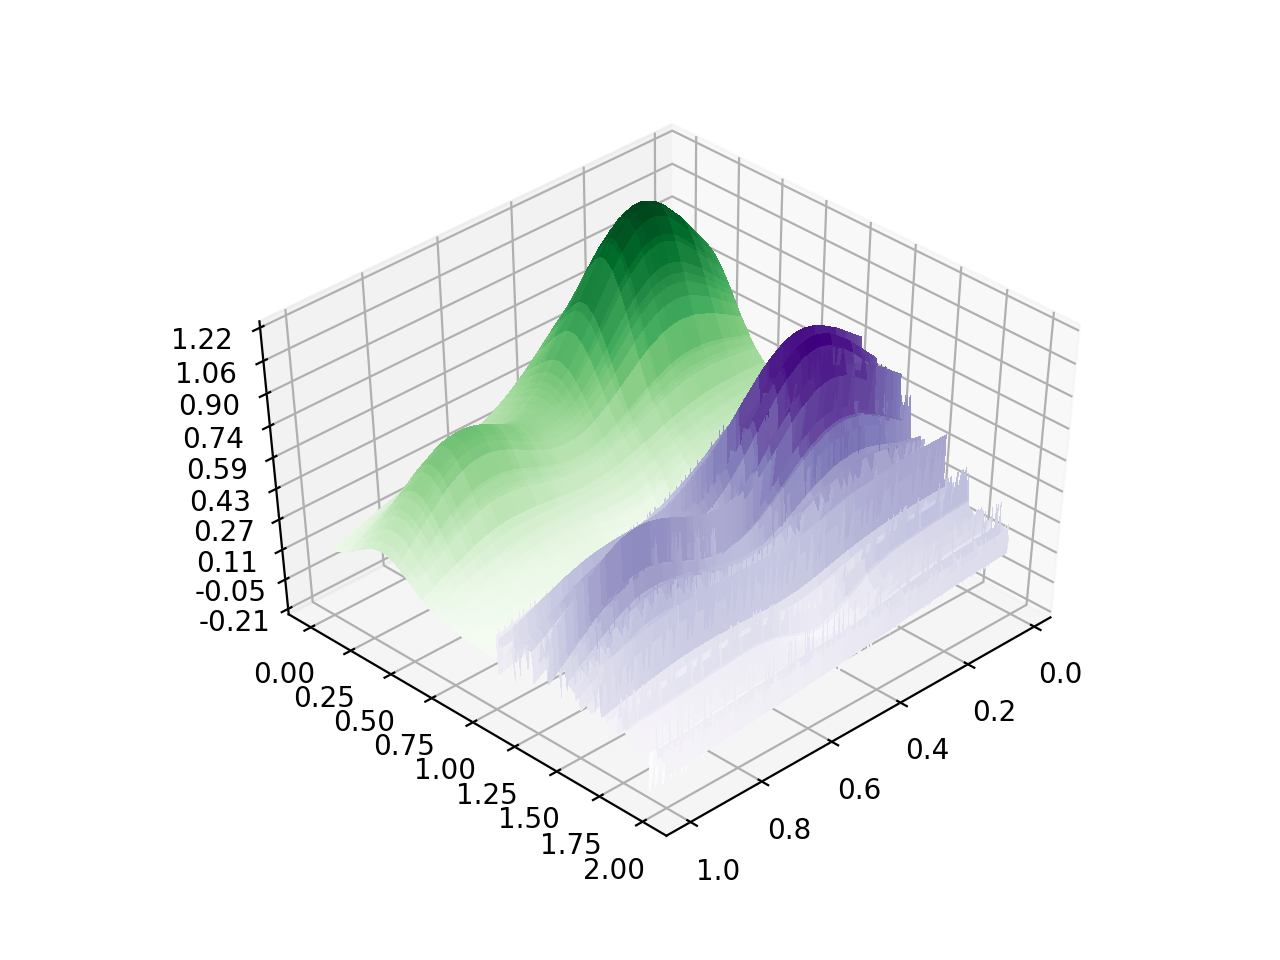
\includegraphics[width=\linewidth]{result/bilder/Franke_noise.png}
        	\caption{}
     \end{subfigure}
     ~
     \begin{subfigure}{0.45\textwidth}
       	\centering
       	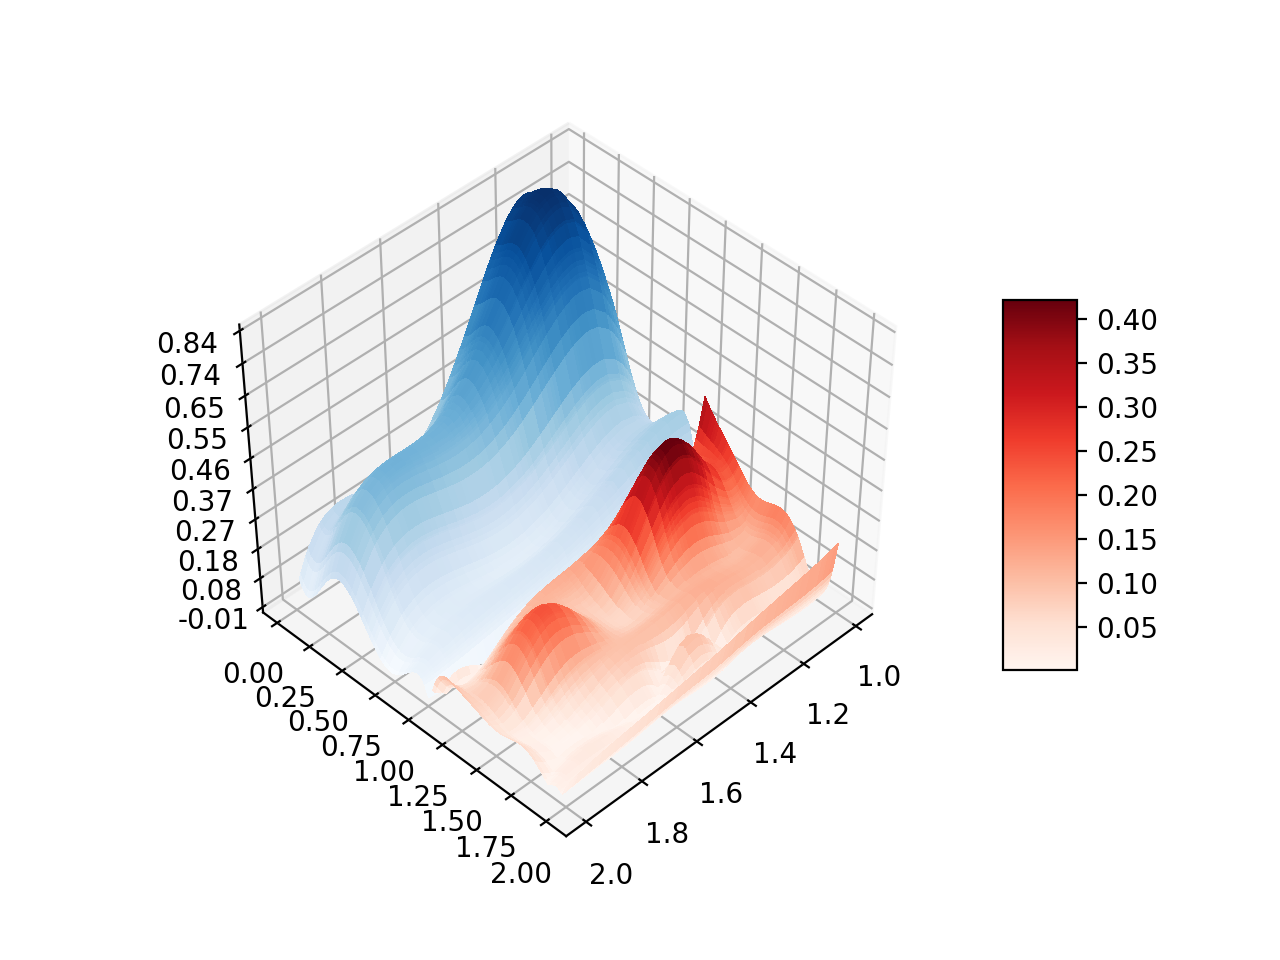
\includegraphics[width=\linewidth]{result/bilder/OLS_bar.png}
        	\caption{}
    	\end{subfigure}
 	\caption{a) \color{green}Franke function \color{black}, and the \color{purple}Frank function with noise plottet\color{black}. b) Our \color{blue}fifth order approximation of the Franke function\color{black}. On the right we have the \color{red}residuals\color{black}, i.e. the error compared to the real function, and its relative size indicated by the red colour gradient.}
	\label{fig:OLS_Frank}
\end{figure}


 \begin{center}
 \label{tab:OLS_Degree_R2_MSE}
 \captionof{table}{MSE and $R^2$ score for OLS by degree. These values are created by taking the average values over 100 different executions, with a noise level $= 0.1$ and a $\lambda = 0.00001$ }
 \begin{tabularx}{\textwidth}{c X c X c  }
     \hline
     \hline
         Degree && R2 && MSE \\
         \hline
2      && 0.71 && 0.01353 \\ 
3      && 0.81 && 0.00916 \\ 
4      && 0.86 && 0.00712 \\ 
5      && 0.88 && 0.00585 \\ \hline
 \end{tabularx}
 \end{center}
 
 \pagebreak
 \begin{center}
 \label{tab:OLS_lambda_R2_MSE}
 \captionof{table}{ MSE and $R^2$ score for OLS by $\lambda$, with a fifth order polynomial. These values are created by taking the average values over $100$ different executions, with a noise level $= 0.1$}
 \begin{tabularx}{\textwidth}{c X c X c  }
     \hline
     \hline
         $\lambda$ && R2 && MSE \\
         \hline
 0.0000001  && 0.87497  && 0.00587 \\
0.0000100  && 0.87517  && 0.00605 \\
0.0010000  && 0.87723  && 0.00592 \\
0.1000000  && 0.87242 && 0.00608 \\
1.0000000  && 0.87708 && 0.00613 \\
2.0000000  && 0.87833 && 0.00586 \\
5.0000000  && 0.87572 && 0.00601 \\
10.0000000 && 0.87528 && 0.00591\\ \hline
 \end{tabularx}
 \end{center}

  \begin{center}
 \label{tab:Confidenceintervall_OLS}
 \captionof{table}{$\beta$, Var and Confidence intervall for OLS by degree of $x$ and $y$. }
 \begin{tabularx}{\textwidth}{c X l X l X l }
     \hline
     \hline
     $x^iy^j$ && $\beta$ && VAR && Confidence intervall \\
     \hline
$x^0y^0$     && 0.259   && 0.001   &&  [0.227, 0.291]     \\ 
$x^0y^1$     && 4.117   && 0.108   &&  [3.788, 4.446]     \\ 
$x^0y^2$     && -18.065 && 2.943   &&  [-19.781, -16.349] \\ 
$x^0y^3$     && 29.764  && 15.934  &&  [25.772, 33.756]   \\ 
$x^0y^4$     && -22.199 && 17.571  &&  [-26.391, -18.007] \\ 
$x^0y^5$     && 6.361   && 2.637   &&  [4.737, 7.985]     \\ 
$x^1y^0$     && 5.277   && 0.074   &&  [5.005, 5.549]     \\ 
$x^1y^1$     && -9.751  && 1.234   &&  [-10.862, -8.64]   \\ 
$x^1y^2$     && 13.591  && 6.186   &&  [11.104, 16.078]   \\ 
$x^1y^3$     && -21.609 && 7.858   &&  [-24.412, -18.806] \\ 
$x^1y^4$     && 12.635  && 1.628   &&  [11.359, 13.911]   \\ 
$x^2y^0$     && -22.726 && 1.825   &&  [-24.077, -21.375] \\ 
$x^2y^1$     && 28.964  && 5.900   &&  [26.535, 31.393]   \\ 
$x^2y^2$     && -1.849  && 6.149   &&  [-4.329, 0.631]    \\ 
$x^2y^3$     && -5.401  && 1.364   &&  [-6.569, -4.233]   \\ 
$x^3y^0$     && 30.056  && 10.123  &&  [26.874, 33.238]   \\ 
$x^3y^1$     && -36.035 && 7.072   &&  [-38.694, -33.376] \\ 
$x^3y^2$     && 6.742   && 1.441   &&  [5.542, 7.942]     \\ 
$x^4y^0$     && -11.919 && 12.008  &&  [-15.384, -8.454]  \\ 
$x^4y^1$     && 12.813  && 1.444   &&  [11.611, 14.015]   \\ 
$x^5y^0$     && -0.909  && 1.951   &&  [-2.306, 0.488]    \\ 

     \hline
 \end{tabularx}
 \end{center}

 
\subsubsection{Ridge regression}
The results from the Ridge calculations are here presented in the same manner as for Ordinary least square. Again finding the MSE, $R^2$ score, according to polynomial degree, and testing for different $\lambda$. Finding the $\beta$ values, VAR, and the Confidence intervall. We see here that the $R^2$ score is unstable for higher values of $\lambda$.
 
 \pagebreak
 \begin{center}
 \label{tab:Ridge_Degree_R2_MSE}
 \captionof{table}{MSE and $R^2$ score for Ridge by degree. These values are created by taking the average values over 100 different executions, with a noise level $= 0.1$ and a $\lambda = 0.00001$.}
 \begin{tabularx}{\textwidth}{c X c X c  }
     \hline
     \hline
         Degree && R2 && MSE \\
         \hline
2      && 0.71 && 0.01353 \\ 
3      && 0.80 && 0.00968 \\ 
4      && 0.81 && 0.00928 \\ 
5      && 0.81 && 0.00902 \\ \hline
 \end{tabularx}
 \end{center}
 
 
\begin{center}
 \label{tab:OLS_lambda_R2_MSE}
 \captionof{table}{ MSE and $R^2$ score for Ridge $\lambda$. These values are created by taking the average values over $100$ different executions, with a noise level $= 0.1$.}
 \begin{tabularx}{\textwidth}{c X c X c  }
     \hline
     \hline
         $\lambda$ && R2 && MSE \\
         \hline
 0.0000001  && 0.81150  && 0.00894 \\
0.0000100  && 0.80979  && 0.00932 \\
0.0010000  && 0.74059  && 0.01237 \\
0.1000000  && -0.20901 && 0.05933 \\
1.0000000  && -1.85170 && 0.13474 \\
2.0000000  && -1.83823 && 0.14025 \\
5.0000000  && -1.79681 && 0.13813 \\
10.0000000 && -1.81950 && 0.13576\\ \hline
 \end{tabularx}
 \end{center}


  \begin{center}
 \label{tab:Confidenceintervall_Ridge}
 \captionof{table}{$\beta$, Var and Confidence intervall for Ridge by degree of $x$ and $y$. }
 \begin{tabularx}{\textwidth}{c X l X l X l }
     \hline
     \hline
     $x^iy^j$ && value && variance && Confidence intervall \\
     \hline
$x^0y^0$     && 0.384    && 0.001   && [0.352, 0.416]     \\
$x^0y^1$     && 1.770    && 0.077   && [1.493, 2.047]     \\
$x^0y^2$     && -0.294   && 1.953   && [-1.691, 1.103]    \\
$x^0y^3$     && -22.690  && 10.474  && [-25.926, -19.454] \\
$x^0y^4$     && 41.542   && 12.033  && [38.073, 45.011]   \\
$x^0y^5$     && -20.675  && 1.949   && [-22.071, -19.279] \\
$x^1y^0$     && 5.348    && 0.068   && [5.087, 5.609]     \\
$x^1y^1$     && -11.544  && 1.040   && [-12.564, -10.524] \\
$x^1y^2$     && 18.567   && 4.891   && [16.355, 20.779]   \\
$x^1y^3$     && -27.573  && 6.071   && [-30.037, -25.109] \\
$x^1y^4$     && 14.943   && 1.295   && [13.805, 16.081]   \\
$x^2y^0$     && -21.987  && 1.712   && [-23.295, -20.679] \\
$x^2y^1$     && 32.153   && 5.221   && [29.868, 34.438]   \\
$x^2y^2$     && -5.093   && 5.179   && [-7.369, -2.817]   \\
$x^2y^3$     && -3.142   && 1.161   && [-4.219, -2.065]   \\
$x^3y^0$     && 25.775   && 9.426   && [22.705, 28.845]   \\
$x^3y^1$     && -39.259  && 6.976   && [-41.9, -36.618]   \\
$x^3y^2$     && 6.673    && 1.214   && [5.571, 7.775]     \\
$x^4y^0$     && -4.833   && 11.244  && [-8.186, -1.48]    \\
$x^4y^1$     && 14.552   && 1.590   && [13.291, 15.813]   \\
$x^5y^0$     && -4.681   && 1.908   && [-6.062, -3.3]    \\ 
    \hline
 \end{tabularx}
 \end{center}      

 

\subsubsection{Lasso regression}
The results from the Lasso regression, again presenting the MSE, $R^2$, $\beta$, VAR, and Confidence interval.


 \begin{center}
 \label{tab:Lasso_Degree_R2_MSE}
 \captionof{table}{MSE and $R^2$ score for Lasso by degree. These values are created by taking the average values over 100 different executions, with a noise level $= 0.1$ and a $\lambda = 0.00001$}
 \begin{tabularx}{\textwidth}{c X c X c  }
     \hline
     \hline
         Degree && R2 && MSE \\
         \hline
2      && 0.71 && 0.01353 \\ 
3      && 0.81 && 0.00916 \\ 
4      && 0.86 && 0.00712 \\ 
5      && 0.88 && 0.00585 \\ \hline
 \end{tabularx}
 \end{center}
 
 
 \begin{center}
 \label{tab:Degree_R2_MSE}
 \captionof{table}{MSE and $R^2$ score for Lasso on Franke function by $\lambda$. These values are created by taking the average values over 100 different executions, with a noise level $= 0.1$}
 \begin{tabularx}{\textwidth}{c X c X c  }
     \hline
     \hline
$\lambda$    &&R2     &&MSE     \\
         \hline
0.0000001 &&0.87497&&0.00587 \\
0.0000100 &&0.87517&&0.00605 \\
0.0010000 &&0.87723&&0.00592 \\
0.1000000 &&0.87242&&0.00608 \\
1.0000000 &&0.87708&&0.00613 \\
2.0000000 &&0.87833&&0.00586 \\
5.0000000 &&0.87572&&0.00601 \\
10.0000000 && 0.87528&&0.00591
 \end{tabularx}
 \end{center}
 
 \begin{center}
\label{tab:lasso-var-conf}
\captionof{table}{$\beta$, Var and Confidence intervall for Ridge by degree of $x$ and $y$. We have here cut the values for higher degrees because these were equal to zero.}
\begin{tabularx}{\textwidth}{c X c X c X l}
    \hline
    \hline
        $x^iy^j$ && $\beta$ && VAR && Confidens interval\\
    \hline
        $x^0y^0$ && 0.342129   && 0.000080   && [0.333197,0.351061] \\
        $x^0y^1$ && -0.437389  && 0.000347   && [-0.456013,-0.418765] \\
        $x^0y^2$ && -0.016612  && 0.000261   && [-0.032765,-0.000458] \\
        $x^0y^5$ && 0.000024   && 0.000000   && [-0.000140,0.000188] \\
        $x^1y^0$ && 0.558845   && 0.000299   && [0.541543,0.576146] \\
        $x^1y^1$ && -0.389778  && 0.000394   && [-0.409623,-0.369933] \\
        $x^3y^0$ && -0.000178  && 0.000001   && [-0.000933,0.000576] \\
        $x^4y^0$ && -0.120878  && 0.000436   && [-0.141758,-0.099998] \\
    \hline
\end{tabularx}
\end{center}


 
\subsection{Ordinary least square, Ridge, and Lasso regression with resampling, now on real data}
In this section we present the OLS, Ridge and Lasso regression on the real data.
\begin{figure}[H]
		\centering
		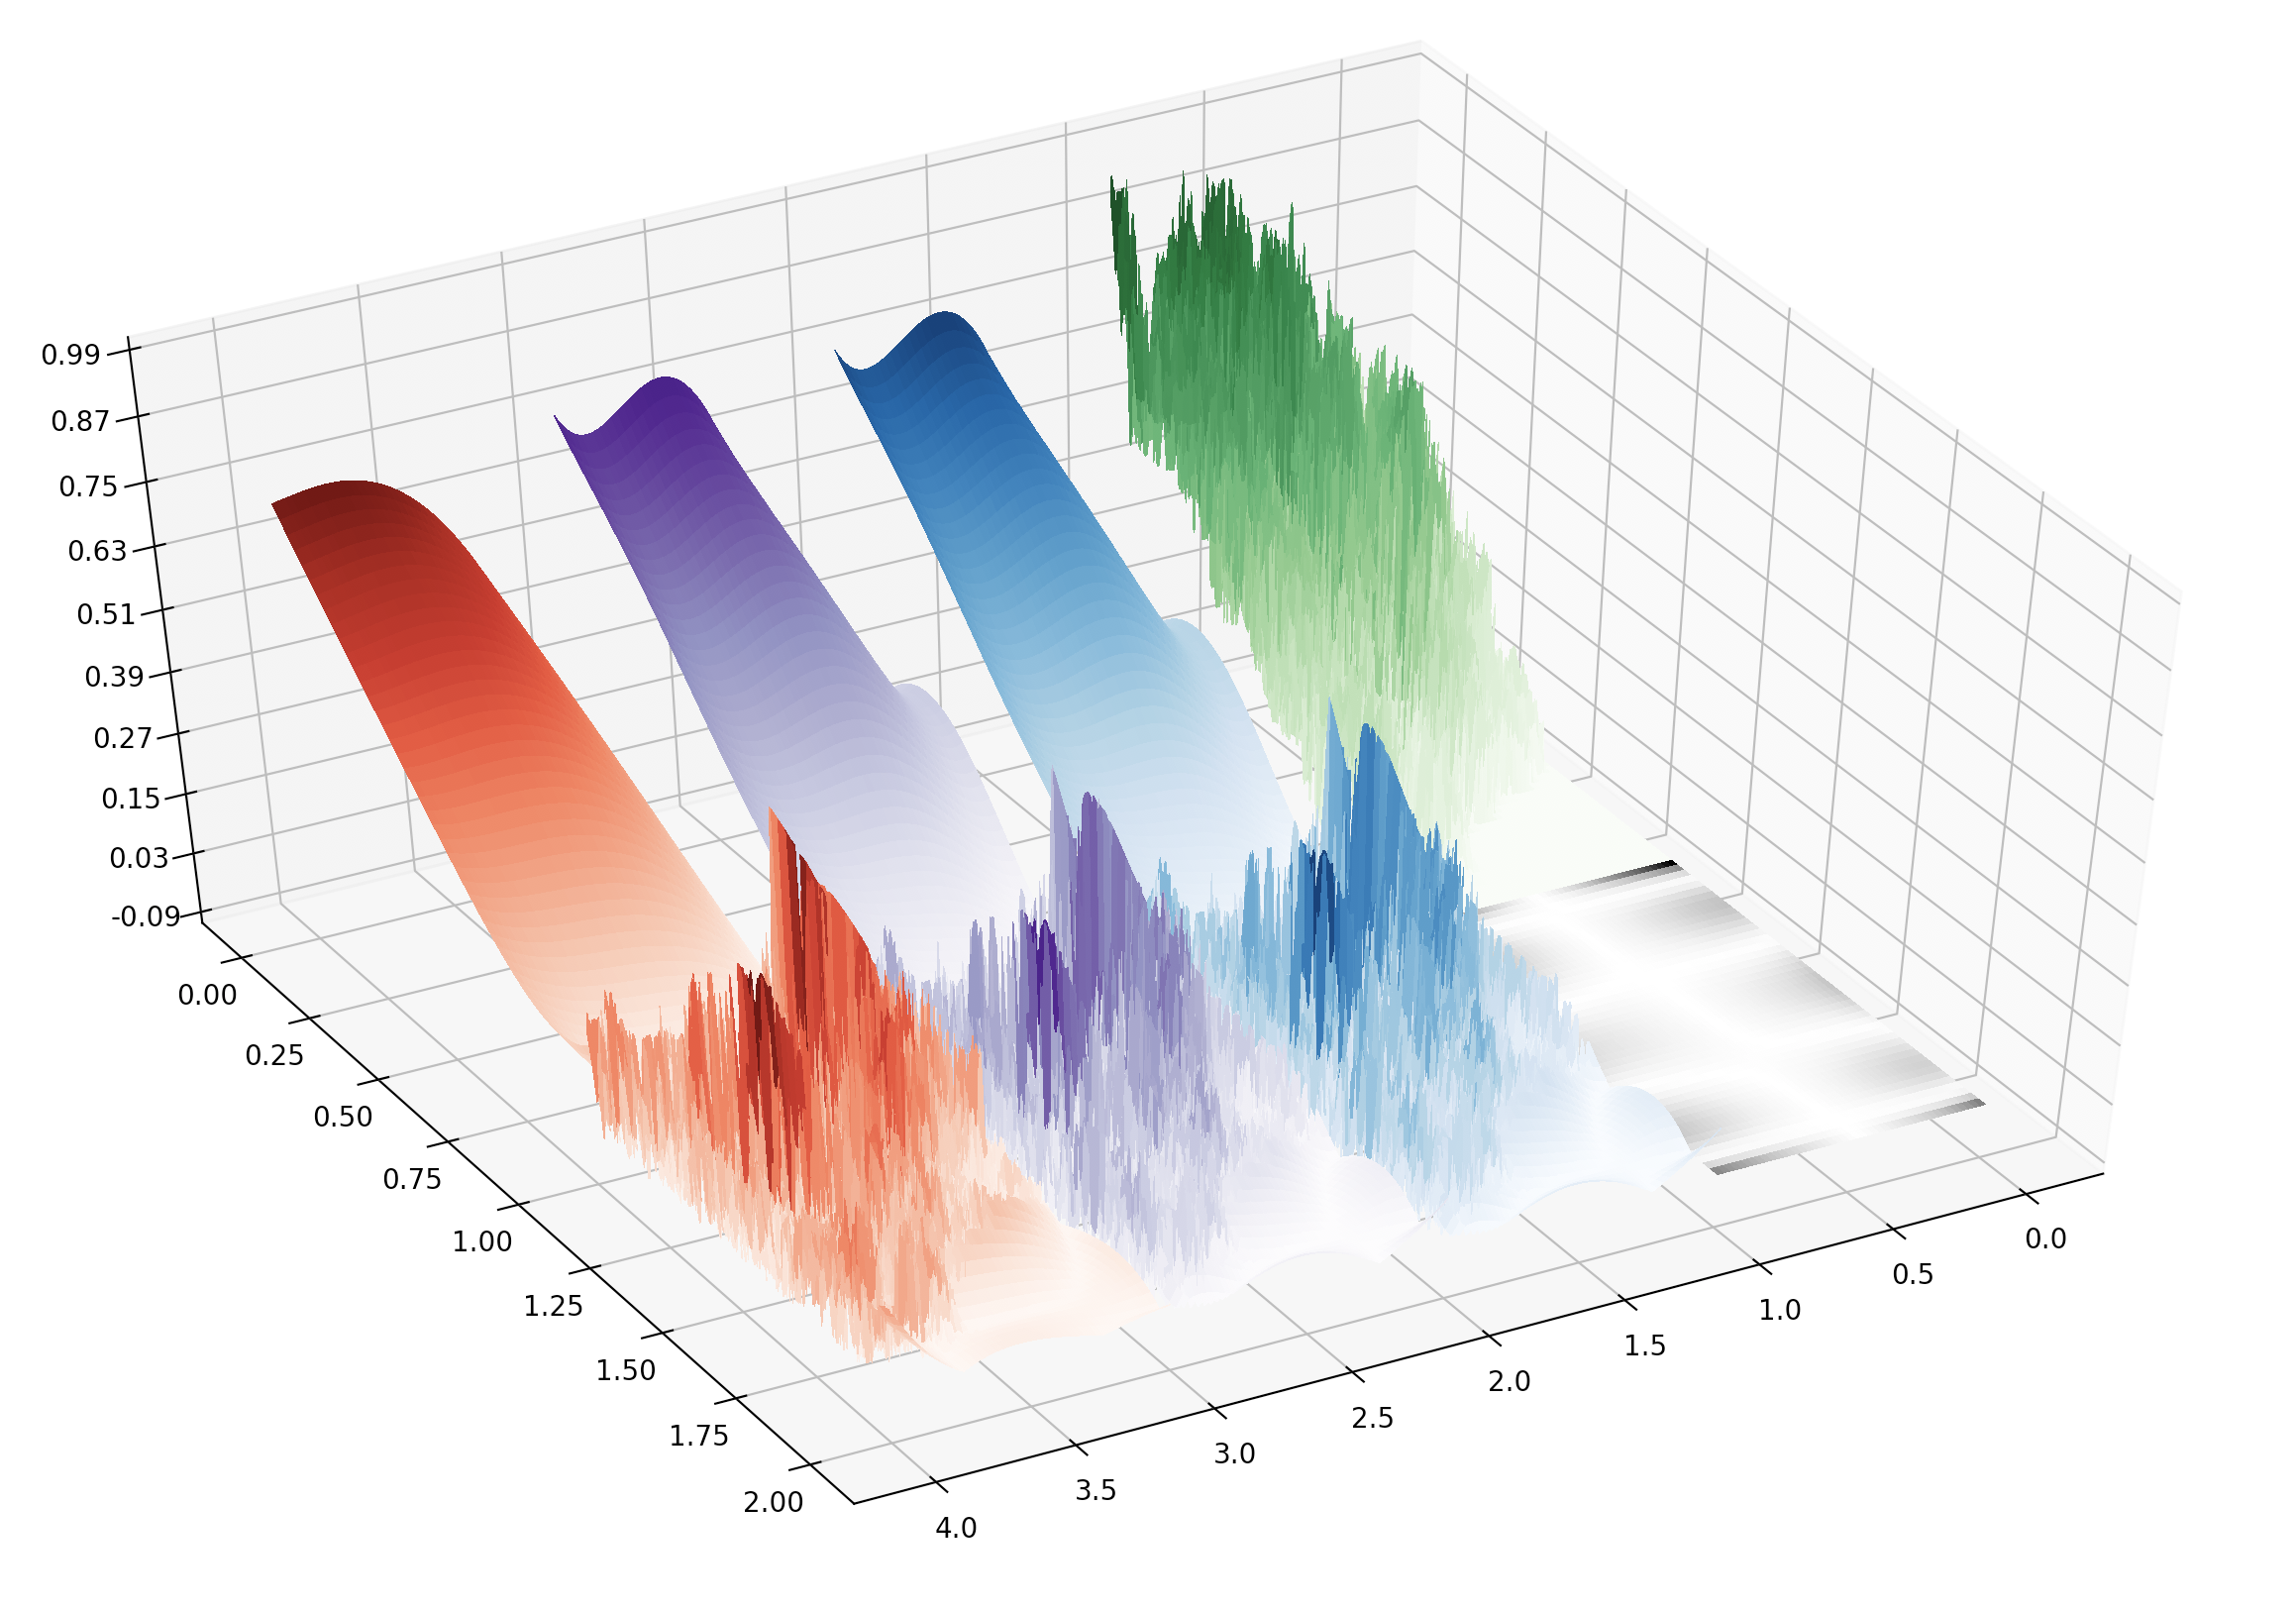
\includegraphics[width=1.1\linewidth]{result/bilder/all_real.png}
		\caption{From left to right: The \color{red}OLS \color{black} regression, \color{purple}{} Ridge \color{black} regression, \color{blue} Lasso \color{black} regression, and the \color{green}Real data \color{black} that we tried to approximate, with their residuals.}
		\label{fig:RealData}
\end{figure}


 \begin{center}
 \label{tab:Realdata_OLS_lambda_R2_MSE}
 \captionof{table}{OLS regression on Real data. }
 \begin{tabularx}{\textwidth}{c X c X c  }
     \hline
     \hline
$\lambda$    &&R2     &&MSE     \\
         \hline
0.0000001 && 0.823088 && 0.010720 \\
0.0000100 && 0.823088 && 0.010720 \\
0.0010000 && 0.823088 && 0.010720 \\
0.1000000 && 0.823088 && 0.010720 \\
 \end{tabularx}
 \end{center}
 
\pagebreak
 
 \begin{center}
 \label{tab:Realdata_Lasso_lambda_R2_MSE}
 \captionof{table}{Lasso on realdata. We saw that $R^2$ got out of hand with a $\lambda = 0.1$ and higher, and decided not to include those numbers. }
 \begin{tabularx}{\textwidth}{c X c X c  }
     \hline
     \hline
$\lambda$    &&R2     &&MSE     \\
         \hline
0.0000001 && 0.797486 && 0.012272 \\
0.0000100 && 0.797470 && 0.012273 \\
0.0010000 && 0.753280 && 0.014950 \\
0.1000000 && -0.165026 && 0.070596 \\
 \end{tabularx}
 \end{center}

 \begin{center}
 \label{tab:Realdata_Ridge_lambda_R2_MSE}
 \captionof{table}{Ridge on realdata. MSE and $R^2$ score for Ridge on the real data by $\lambda$. }
 \begin{tabularx}{\textwidth}{c X c X c  }
     \hline
     \hline
$\lambda$    &&R2     &&MSE     \\
         \hline
0.0000001 && 0.823088 && 0.010720 \\
0.0000100 && 0.823088 && 0.010720 \\
0.0010000 && 0.823027 && 0.010724 \\
0.1000000 && 0.818116 && 0.011022 \\
 \end{tabularx}
 \end{center}





%Presenter en kristisk vurdering og diskuter applikasjonsmulighetene(applicability) av disse regresjonsmetodene til typen data som blir presentert her. DISKUSJONSDEL



%\pagebreak
\section{Conclusion}




It seems that the SIRS model is a great system dynamics model for representing real diseases, in general a great foundation to build on for predicting disease, in this case, and how they establish themselvs within the population. We have also seen that it is very versatile, with a few improvements tested out, and combined in this report. It was shown that a Monte Carlo simulation were a great way of approaching the differential equations in a more realistic manner, if given a large enough dataset. 


\pagebreak
\section{References:}
note: bibtex did not want to work with me on this project.
\begin{itemize}
\item Yang, Wan, Alicia Karspeck, and Jeffrey Shaman. "Comparison of filtering methods for the modeling and retrospective forecasting of influenza epidemics." PLoS computational biology 10.4 (2014): e1003583.

\item Zaman, Gul, Yong Han Kang, and Il Hyo Jung. "Stability analysis and optimal vaccination of an SIR epidemic model." BioSystems 93.3 (2008): 240-249.

\item Ramachandran, Prajit, Barret Zoph, and Quoc V. Le. "Searching for activation functions." (2018).\label{ref:3}

\end{itemize}


%\pagebreak
%\printbibliography

\section{Appendix}\label{sec:appendix}
\subsection{Supervised Learning, some results:}
\begin{tabular}{|c|c|c|c|c|c|c|} \hline
func	&	node	&	epoch	&	step	&		MSE		&	R2	\\ 
\hline
swis	&	100 	&	100 	& 	01 		&	4301.860	&	-1.504686		\\ 
\hline
swis	&	100 	&	100 	& 	001		&	4383.970	&	-0.062676		\\ 
\hline
swis	&	100 	&	100  	& 	0001	&	18649.730	&	-1612.388089		\\ 
\hline
swis	&	100 	&	1000 	& 	01		&	5405.858	&	-0.947049		\\ 
\hline
swis	&	100 	&	1000	& 	001		&	4996.257	&	-1.148733		\\ 
\hline
swis	&	100 	&	1000	& 	0001	&	4068.276	&	-0.079732		\\ 
\hline
swis	&	100 	&	10000	& 	01		&	 5405.352	&	 -0.946243		\\ 
\hline
swis	&	100 	&	10000	& 	001		&	 5405.650	&	 -0.946284		\\ 
\hline
swis	&	100 	&	10000	& 	0001 	&	5395.676 	& -0.955657		\\ 
\hline
swis	&	1000	&	 100	& 	01		&	 5344.535	&	 -0.9690825\\ 
\hline
swis	&	1000	&	 100	& 	001		&	 4301.586	&	 -1.5146678\\ 
\hline
swis	&	1000	&	 100	& 	0001	&	 7687.034	&	 -7.0514296\\ 
\hline
swis	&	1000	&	 1000	& 	01		&	 5406.056	&	 -0.9465423\\ 
\hline
swis	&	1000	&	 1000 	& 	001		&	 5405.020	&	 -0.9540634\\ 
\hline
swis	&	1000	&	 1000 	&	 0001	&	 4381.460	&	 -1.5773855\\ 
\hline
swis	&	1000	&	 10000 	&  	01		&	 5408.282	&	 -0.9504758\\ 
\hline
swis	&	1000	&	 10000 	&	 001	&	 5405.543	&	 -0.9462314\\ 
\hline
swis	&	1000	&	 10000 	&	 0001	&	 5407.491	&	 -0.9473403\\ 
\hline
tan 	& 100 		&   100   	& 	01		&	 4722.055 	&	-1.4382791	\\ 
\hline
tan 	& 100  		&	100   	& 	001		&	 4541.822 	&	-63.0650826	\\ 
\hline
tan 	& 100  		&	100   	& 	0001	&	 18327.134	&	 -2164.3759400 	\\ 
\hline
tan 	& 100  		&	1000  	& 	01		&	 5389.155 	&	-0.9489306     \\
\hline
tan 	& 100  		&	1000  	& 	001		&	 4560.229 	&	-1.4495536   	\\ 
\hline
tan 	& 100  		&	1000  	&	 0001	&	 4609.627 	&	-47.9667788	\\ 
\hline
tan 	& 100  		&	10000 	& 	01 		&	5406.032	&	 -0.9464465	\\ 
\hline
tan 	& 100  		&	10000 	& 	001 	&	5405.054	&	 -0.9468466	\\ 
\hline
tan 	& 100  		&	10000 	& 	0001 	&	5136.405	&	 -1.0999677	\\ 
\hline
tan 	& 1000 		&	 100  	& 	01 		&	5301.474	&	 -1.0137502	\\ 
\hline
tan 	& 1000 		&	 100  	& 	001 	&	4726.264	&	 -1.5468762	\\ 
\hline
tan 	& 1000 		&	 100  	& 	0001 	&	6837.188 	&	-10.2774431	\\ 
\hline
tan 	& 1000 		&	 1000 	 & 	01		&	 5408.170	&	 -0.9473984	\\ 
\hline
tan 	& 1000 		&	 1000 	 & 	001 	&	5401.553 	&	-0.9657959\\ 
\hline
tan 	& 1000 		&	 1000 	 & 	0001	&	 4568.399	&	 -1.4008756\\ 
\hline
tan 	& 1000 		&	 10000	 & 	01		&	 5530.394	&	 -0.9048310\\ 
\hline
tan 	& 1000 		&	 10000	 & 	001		&	 5408.057	&	 -0.9453489\\ 
\hline
tan 	& 1000 		&	 10000	 & 	0001	&	 5408.827	&	 -0.9476682\\ 
\hline
arctan& 100 &100	& 01& 4695.224& -1.3245204	\\ 
\hline
arctan& 100 &100	& 001 &3061.016 & -6.1246861	\\ 
\hline
arctan& 100 &100	& 0001 &18306.907& -1982.2542040	\\ 
\hline
arctan& 100 &1000 	&01 &5353.242& -0.9334961	\\ 
\hline
arctan& 100 &1000	& 001 &4352.663& -1.4293472	\\ 
\hline
arctan& 100 &1000	& 0001 &3198.084& -5.7849874	\\ 
\hline
arctan& 100 &10000	& 01 &5409.115& -0.9443223		\\ 
\hline
arctan& 100 &10000	& 001 &5399.718& -0.9443793	\\ 
\hline
arctan& 100 &10000 	&	0001 &5029.071 &-1.0632415	\\ 
\hline
arctan& 1000& 100 	&01& 5102.813& -1.0711406	\\ 
\hline
arctan& 1000& 100 	&001 &4579.046& -1.4685736	\\ 
\hline
\end{tabular}

See github.come/sondrt/






%\begin{align*}
%&n \qquad &2^n - (-1)^n\\
%&n+1 \qquad &2^{n+1} - (-1)^{n+1} \\
%& &= 2(2^{n}) - (-1)^{n+1}\\
%& &= 2(2^{n} + (-1)^n  + (-1)^{n+1}) - (-1)^{n+1}\\
%& &= 2(2^{n} + (-1)^n  - (-1)^{n}) - (-1)^{n+1}\\
%& &= 2(2^{n}- (-1)^{n}) + 2(-1)^n  + (-1)^{n}\\
%& &= 2(2^{n}- (-1)^{n}) + 3(-1)^n \\
%\end{align*}



% \begin{figure}[H]
%     \centering
%     \begin{subfigure}{0.5\textwidth}
%         \centering
%         \includegraphics[width=\linewidth]{result/bilder/Tc/e-Tc}
%         \caption{}
%     \end{subfigure}%
%     ~ 
%     \begin{subfigure}{0.5\textwidth}
%         \centering
%         \includegraphics[width=\linewidth]{result/bilder/Tc/m-Tc}
%         \caption{}
%     \end{subfigure}
%     \caption{a) Shows how E behaves around $T_C$ b) Shows how |M| develops near $T_C$.}
%     \label{fig:tc-E-M}
% \end{figure}






% \begin{center}
% \label{tab:states-2x2-summary}
% \captionof{table}{The table shows a summary from table \ref{tab:states-2x2}. }
% \begin{tabularx}{\textwidth}{c X c X c X c}
%     \hline 
%     \hline 
%         Number of $\color{red}{\uparrow}$ && Multiplicity && Energy && Magnetic moment \\ 
%     \hline
%         4   &&      1      &&      -8J     &&       4       \\  
%         3   &&      4      &&      0J      &&       2       \\
%         2   &&      2      &&      8J      &&       0       \\
%         2   &&      4      &&      0J      &&       0       \\
%         1   &&      4      &&      0J      &&       -2      \\
%         0   &&      1      &&      -8J     &&       -4      \\
%     \hline
% \end{tabularx}
% \end{center}




%\begin{tabular}{|c|c|c|c|c|c|c|}
%	\hline 
%	n & General & Specific & LU & fastest & slowest & $\frac{slowest}{fastest}$\\ 
%	\hline
%	10 & 6.5e-05 & 5e-06 & 4e-05 & Specific & General & 13.0\\ 
%	\hline 
%	100 & 7.5e-05 & 8e-06 & 0.0023 & Specific & LU & 287.5\\ 
%	\hline 
%	1000 & 0.00014 & 4e-05 & 0.26 & Specific & LU & 6500\\ 
%	\hline
%	10000 & 0.0007 & 0.0005 & 142.5 & Specific & LU & 285000 \\ 
%	\hline
%\end{tabular}

%\begin{figure}[H]
%		\centering
%		\includegraphics[width=0.7\linewidth]{ab.png}
%		\caption{Atomene er gule kuler, de elementære vektorene er blå og a vektorene er grønne.}
%		\label{fig:ab}
%\end{figure}















\end{document}